XFunctions extends XElements.

This class is the heart of the code (netlist) generation. It has methods
which use the Elements created in class XElements to provide higher
level functions such as registers, multiplexers and queue buffers.

The following functional elements are implemented by methods
in this class -

\blist
\item   registers - to implement static mode variables and to provide
        registers for other methods in this class
\item   resynchroniser - to transfer a pulse from one clock domain to
        another
\item   queue buffers - to implement queue mode variables
\item   delay line - to implement the TDEDEL intermediate code element
\item   shifters - to implement left and right constant and variable
        shift
\item   adder - to implement addition
\item   inverter - to implement bit inversion
\item   incrementer - to implement addition by 1
\item   subtracter - to implement subtraction
\item   decrementer - to implement subtraction by 1
\item   adder/subtracter - to implement selectable addition or
        subtraction
\item   ALU - to implement addition/subtraction/assignment in CLBs
\item   incrementer/decrementer - to implement selectable addition or
        subtraction of 1
\item   signed and unsigned multipliers - to implement multiplication
        using hardware if available and CLB logic otherwise
\item   signed and unsigned divider/remainder - to implement to
        implement division and remaindering using CLB logic
\item   numerical comparators - to implement equal, not equal,
        greater than, greater than or equal, less than and less than or
        equal numerical comparisons
\item   combinatorial RAM and ROM - to implement cmemory mode variables
\item   registered output RAM - to implement rmemory mode variables
\blend

\subsection{registers}

    \begin{lstlisting}[gobble=4, language=java]
        public Net[] reg (
            Net[]               in,
            Net                 c,
            Net                 ce,
            Net                 r,
            String              sinit,
            ArrayList<String>   constraints
        ) {
            int                 width = in.length;
            Net[]               out = new Net[width];
            ArrayList<String>   locs = new ArrayList<String>();

            // Constraints here are single strings -
            //  "TNM=..."
            //  "LOC=..."
            //  "DSP"
            // having been modified in XTDECode.TDEREG() from the key=value pairs
            // in the original TDE list.
            // Location constraints should be one per bit.
            // The DSP constraint is ignored.
            if (constraints != null) {
                Iterator<String>    it = constraints.iterator();
                while (it.hasNext()) {
                    String s = it.next();
                    if (s.startsWith("LOC=")) {
                        locs.add(s);
                        it.remove();
                    }
                }
            }
            if (sinit == null)
                sinit = "0";
            for (int bit=0 ; bit<width ; bit++) {
                if (!locs.isEmpty())
                    constraints.add(0, locs.get(0));
                if ((strhexbit(sinit, bit) & 1) == 0)
                    out[bit] = FDRS(in[bit], c, ce, r, null, "R", constraints);
                else
                    out[bit] = FDRS(in[bit], c, ce, null, r, "S", constraints);
                if (!locs.isEmpty()) {
                    locs.remove(0);
                    constraints.remove(0);
                }
            }
            return(out);
        }
    \end{lstlisting}
    This method creates a register which has a single clock enable and
    single reset common to all flip-flops in the register. It is called
    from XTDECode.TDEREG() to create a static mode variable that is one
    bit wide and from several methods in this class to create registers.
    It is only in the former case that the constraints argument will be
    non-null.

    The code first searches the constraints list for location
    constraints (they start with "LOC="). It removes these, copying them
    to a new list. As each bit is created a location constraint is
    copied from the list (if there are any) and is put back at the
    front of the constraints list. At the end of the loop that location
    constraint is removed from both lists.

    If there is no initialisation string the string "0" is assigned.

    For each register bit the appropriate bit is extracted from the
    initialisation string using method strhexbit() from class
    genFunctions. Method FDRS() from class XElements is then called
    with either an "R" or "S" property argument and the reset signal
    is connected to either the R or S input as appropriate.

    \begin{lstlisting}[gobble=4, language=java]
        public Net[] reg (
            Net[]       in,
            Net         c,
            Net[]       ce,
            Net[]       r,
            String      sinit,
            ArrayList   constraints
        ) {
            int         width = in.length;
            Net[]       out = netArray(width);
            ArrayList   locs = new ArrayList();
            boolean     dsp = false;

            .
            . code for use of multiplier/DSP register
            .

            if (sinit == null)
                sinit = "0";
            out = new Net[width];
            for (int bit=0 ; bit<width ; bit++) {
                if (!locs.isEmpty())
                    constraints.add(0, (String)locs.get(0));
                if ((strhexbit(sinit, bit) & 1) == 0)
                    out[bit] = FDRS(in[bit], c, ce[bit], r[bit], null, "R", constraints);
                else
                    out[bit] = FDRS(in[bit], c, ce[bit], null, r[bit], "S", constraints);
                if (!locs.isEmpty()) {
                    locs.remove(0);
                    constraints.remove(0);
                }
            }
            return(out);
        }
    \end{lstlisting}
    This method differs from the previous in two respects -
    \blist
    \item   if there is no DSP constraint it is very similar to the
            previous method except that the clock enable and reset signals
            are now arrays, one for each flip-flop, rather than common
            single signals
    \item   if there is a DSP constraint, the register is not
            initialised and the FPGA has a hardware multiplier or DSP block
            then the register is implemented using the output register
            of a multiplier or DSP block
    \blend

    A map, {\bf hm}, and two classes, {\bf Cer} and {\bf Group}, were
    defined in the method for use when a DSP constraint is acted upon.
    These are used to group flip-flops within the register which share
    the same clock enable and reset signals. Each such group is
    implemented in a separate multiplier or DSP block since the clock
    enables and resets are common to all bits in those hardware
    registers. If a group entry is larger than the width of the hardware
    register then multiple units will be used. The {\bf Cer} class contains a
    Net pair, a clock enable and a reset. These are used as the key to
    map {\bf hm} which thus has an entry for each unique pair. The
    associated map value is class {\bf Group} which has an input list and an
    output list. These contain the input and output signals of
    flip-flops in each CE/R group in LSB to MSB bit order.

    The declarations are -
    \begin{lstlisting}[gobble=4, language=java]
        HashMap     hm = null;
        class Cer {
            Net ce;
            Net r;

            Cer (Net ce, Net r) {
                this.ce = ce;
                this.r = r;
            }

            public boolean equals (Object o) {
                return(ce.equals(((Cer)o).ce) && r.equals(((Cer)o).r));
            }
            public int hashCode () {
                return((ce.hashCode() << 16) + r.hashCode());
            }
        }
        class Group {
            ArrayList   inputs = new ArrayList();
            ArrayList   outputs = new ArrayList();
        }
    \end{lstlisting}
    The equals() and hashCode() methods are implemented to enable
    correct functioning of HashMap keys.

    The code to create the group data structure is -
    \begin{lstlisting}[gobble=4, language=java]
        hm = new HashMap();
        for (int i=0 ; i<width ; i++) {
            Cer x = new Cer(ce[i], r[i]);
            if (!hm.containsKey(x))
                hm.put(x, new Group());
            Group g = (Group)hm.get(x);
            g.inputs.add(in[i]);
            g.outputs.add(out[i]);
        }
    \end{lstlisting}

    The code to create the register is -
    \begin{lstlisting}[gobble=4, language=java]
        Iterator    mit = hm.entrySet().iterator();
        while (mit.hasNext()) {
            Map.Entry   me = (Map.Entry)mit.next();
            Cer         cer = (Cer)me.getKey();
            Group       g = (Group)me.getValue();
            Net[]       gout = new Net[1];
            Net[]       gin = new Net[1];
            int         gwidth = gout.length;
            int         mwidth = DSPRegWidth();
            int         k;
            int         l = gwidth;
            gout = (Net[])g.outputs.toArray(gout);
            gin = (Net[])g.inputs.toArray(gin);

            for (int j=0 ; j<gwidth ; j+=mwidth, l-=mwidth) {
                k = (l >= mwidth) ? j + mwidth - 1 : j + l - 1;
                MULREG(subarray(gin, j, k), subarray(gout, j, k), c, cer.ce, cer.r);
            }
        }
        return(out);
    \end{lstlisting}
    This iterates through the entries in the map converting each group
    into a register using one or more multipliers or DSP blocks. The
    cell type of Element(s) produced is MULREG which is later converted
    to MULT18X18 or DSP48E depending on the FPGA type (method {\bf
    convertElements()} in classes {\bf XC2VP}, {\bf XC5V} etc.).


\subsection{resynchroniser}

    A resynchroniser generates a pulse in another clock domain from a
    rising edge. When the input rises the rise is captured by the next
    input clock edge and an output pulse of one period duration is
    generated on the next output clock edge. This method is used
    by intermediate code TDE {\bf TDERESYNC} and also indirectly by
    methods {\bf async\_buffer()} and {\bf triggerbuffer(}) (via
    {\bf asynch\_fifo\_control()}) in this class.

    The logic circuit used is -

    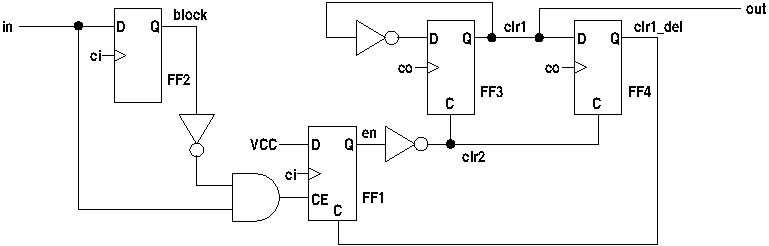
\includegraphics{resync}

    Note that FF1, FF3 and FF4 have asynchronous clear inputs. Initially
    all flip-flop outputs are low, thus {\bf block} and {\bf clr1}/{\bf
    out} are low. When {\bf in} goes high both FF1 and FF2 outputs go
    high on the next edge of clock {\bf ci}, the input clock. The {\bf
    CE} input of FF1 goes low as {\bf block} is now high. Since {\bf en}
    is now high, {\bf clr2} is low and this enables FF3 to toggle on the
    next edge of {\bf co}, the output clock, raising the output {\bf
    out}. On the next edge of {\bf co} FF3 toggles low again and FF4 is
    set, raising {\bf clr1\_del}, which clears FF1. When {\bf en} thus
    goes low {\bf clr2} goes high clamping FF3 low and clearing FF4. FF1
    is now free to again latch an input however if {\bf in} is still
    high {\bf block} will disable FF1. Thus {\bf in} must be clocked low
    to lower {\bf block} before FF1 can again start the pulse cycle.
    This circuit avoids race conditions between flip-flops in the two
    clock domains.

    The code to generate this is -

    \begin{lstlisting}[gobble=4, language=java]
        public Net resync (Net in, Net ci, Net co) {
            Net en;
            Net block;
            Net clr1 = new Net();
            Net clr1_del = new Net();
            Net clr2;

            block = FDRS(in, ci, null, null, null, null, null);
            en = FDCP(Net.HI, ci, AND(in, INV(block)), clr1_del, null, null, null);
            clr2 = INV(en);
            clr1.connect(FDCP(INV(clr1), co, null, clr2, null, null, null));
            clr1_del.connect(FDCP(clr1, co, null, clr2, null, null, null));
            return(clr1);
        }
    \end{lstlisting}
    Note the use of the connect() method. For example in the statement
    \begin{lstlisting}[gobble=4, language=java]
        clr1.connect(FDCP(INV(clr1), co, null, clr2, null, null, null));
    \end{lstlisting}
    the output Net is also used as an input argument, i.e. there is
    feedback. Thus the Net {\bf clr1} is declared and assigned a new
    instance, then passed as an input argument. The result returned from
    the call is then connected to Net {\bf clr1}. It cannot be assigned
    as that would overwrite the previous Net instance. A similar though
    more indirect argument applies to Net {\bf clr1\_del}.



\subsection{queue buffers}

    These were described in some detail in the section on intermediate
    code TDEs. Some of that description is repeated here.

    There are five methods for generating queue buffers -
    \blist
    \item   queuebuffer() - synchronous 2-deep default queue buffer
    \item   sync\_buffer() - synchronous n-deep queue buffer
    \item   async\_buffer() - asynchronous n-deep queue buffer
    \item   triggerbuffer() - synchronous or asynchronous n-deep queue
            buffer with no data
    \item   queueunbuffered() - a synchronous 0-deep queue buffer (no buffer)
    \blend

    \subsubsection{queuebuffer()}

        This method creates a synchronous queue buffer of depth 2.
        The logic for the default synchronous queue buffer of depth
        two is -

        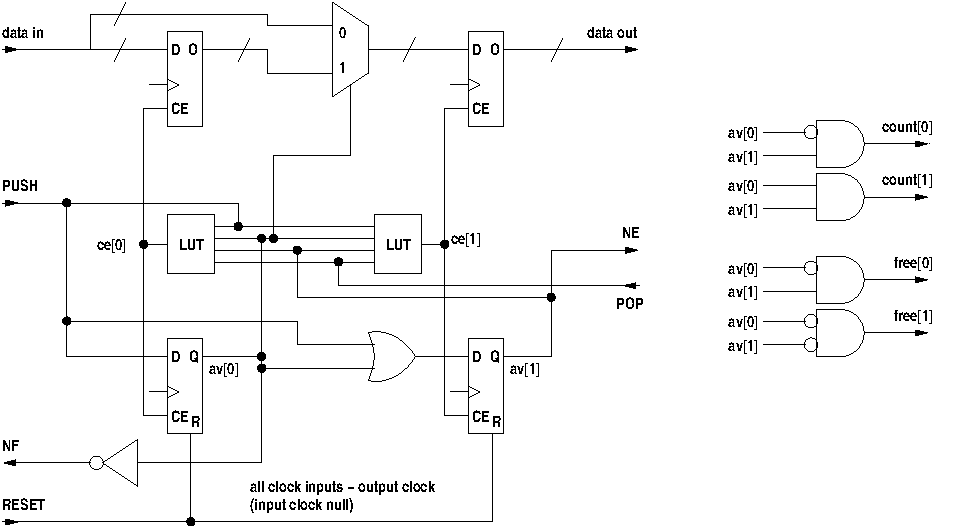
\includegraphics{queuebuffer}

        The 2-input multiplexer shown uses a 3-input LUT per bit.

        When PUSH is high input data is latched into one of two
        registers. If the buffer is empty the data is latched into the
        rightmost register to which the data output is directly
        connected. If another datum is written to the queue buffer it
        goes into the second (left) register. When a datum is popped the
        two registers are shifted right. This scheme avoids having
        combinatorial logic at the output thus minimising
        clock-to-data-out time. The tradeoff is a longer input setup
        time. The two flip-flops represent the occupancy status of the
        two registers. Each register/flip-flop pair has a common clock
        enable controlled by a 4-input LUT.

        The truth table for the control logic is as follows -

        \sf{\small{
        \begin{tabular}{ | c | c | c | c | | c | c | c | | c | c | c | c | c | c | l }
        \cline{1-13}
        \multicolumn{7}{| c ||}{t} & \multicolumn{6}{ c |}{t+1} & \\
        \cline{1-13}
          &    & \multicolumn{2}{ c ||}{av} & \multicolumn{2}{ c |}{ce} & & \multicolumn{2}{ c |}{av}
          & \multicolumn{2}{ c |}{ce} & & & \\
        PUSH & POP & [0] & [1] & [0] & [1] & MUX & [0] & [1] & [0] & [1] & NE & NF & \\
        \cline{1-13}
        \cline{1-13}
        0 & 0 & 0 & 0 & 0 & 0 & X & 0 & 0 & 0 & 0 & 0 & 1 & empty \\
          &   & 0 & 1 & 0 & 0 & X & 0 & 1 & 0 & 1 & 1 & 1 & 1 entry \\
          &   & 1 & 0 & - & - & - & - & - & - & - & - & - & illegal state \\
          &   & 1 & 1 & 0 & 0 & X & 1 & 1 & 1 & 1 & 1 & 0 & full \\
        \cline{1-13}
        0 & 1 & 0 & 0 & - & - & - & - & - & - & - & - & - & illegal state \\
          &   & 0 & 1 & X & 1 & X & 0 & 0 & 0 & 0 & 0 & 1 & av[1] $\downarrow$ POP, now empty\\
          &   & 1 & 0 & - & - & - & - & - & - & - & - & - & illegal state \\
          &   & 1 & 1 & 1 & 1 & 1 & 0 & 1 & 0 & 1 & 1 & 1 & av[0] $\downarrow$ POP, 1 remaining\\
        \cline{1-13}
        1 & 0 & 0 & 0 & 0 & 1 & 0 & 0 & 1 & 0 & 1 & 1 & 1 & av[1] $\uparrow$ PUSH, 1 entry\\
          &   & 0 & 1 & 1 & 0 & X & 1 & 1 & 1 & 1 & 1 & 0 & av[0] $\uparrow$ PUSH, now full\\
          &   & 1 & 0 & - & - & - & - & - & - & - & - & - & illegal state \\
          &   & 1 & 1 & - & - & - & - & - & - & - & - & - & illegal state \\
        \cline{1-13}
        1 & 1 & 0 & 0 & - & - & - & - & - & - & - & - & - & illegal state \\
          &   & 0 & 1 & 0 & 1 & 0 & 0 & 1 & 0 & 1 & 1 & 1 & 1 entry \\
          &   & 1 & 0 & - & - & - & - & - & - & - & - & - & illegal state \\
          &   & 1 & 1 & - & - & - & - & - & - & - & - & - & illegal state \\
        \cline{1-13}
        \end{tabular}
        }}

        {\bf PUSH} must not be raised when
        {\bf NF} is low and {\bf POP} must not be raised when
        {\bf NE} is low.

        The illegal states are described in the following table

        \sf{\small{
        \begin{tabular}{ c | c | c | c | c || l | }
        \multicolumn{6}{ c }{illegal states} \\
        & PUSH & POP & av[0] & av[1]  \\
        \hline
        1 & 0 & 0 & 1 & 0 & single entry must be at righXTDECode extends XFunctions. Its main function is to implement the
abstract methods in class TDECode which generate netlist code from
TDEs. These methods call methods in class xilinx/XFunctions which in
turn call methods in class xilinx/XElements.
t  \\
        2 & 0 & 1 & 0 & 0 & cannot pop when empty  \\
        3 & 0 & 1 & 1 & 0 & single entry must be at right  \\
        4 & 1 & 0 & 1 & 0 & single entry must be at right  \\
        5 & 1 & 0 & 1 & 1 & cannot push when full  \\
        6 & 1 & 1 & 0 & 0 & cannot pop when empty  \\
        7 & 1 & 1 & 1 & 0 & single entry must be at right  \\
        8 & 1 & 1 & 1 & 1 & cannot push when full  \\
        \hline
        \end{tabular}
        }}

        In entries 1, 3, 4 and 7 a single datum in the buffer must
        reside in the right register, so these states are not
        allowed.

        In entry 2 the registers are both empty and so a {\bf POP}
        is not allowed since there is no valid output ({\bf NE} is
        low). The logic has been designed so that no state change
        occurs, i.e. the {\bf POP} is ignored.

        In entry 6 the registers are both empty and so a {\bf POP}
        is not allowed since there is no valid output ({\bf NE} is
        low), however {\bf PUSH} is high. The logic has been designed
        so that the {\bf PUSH} is handled but the {\bf POP} is
        ignored.

        In entries 5 and 8 both registers are full and hence no {\bf
        PUSH} is allowed. Note that this is true even when {\bf POP}
        is asserted since we cannot allow {\bf NF} (not full) to
        depend on {\bf POP} or we generate the very logic cascade
        this buffering scheme was designed to avoid. The logic has
        been designed to ignore {\bf PUSH} in these cases.

        The truth tables for the two LUTs are -

        \sf{\small{
        \begin{tabular}{ l || c | c | c | c |}
        & PUSH & POP & av[0] & av[1]  \\
        \hline
        ce[0] & 0 & 1 & 1 & 1 \\
              & 1 & 0 & 0 & 1 \\
        \hline
        ce[1] & 0 & 1 & X & 1 \\
              & 1 & X & 0 & 0 \\
              & 1 & 1 & 0 & 1 \\
        \hline
        \end{tabular}
        }}

        The code for this is -

        \begin{lstlisting}[gobble=8, language=java]
            public Net[] queuebuffer (
                Net[]   in,     // data input
                Net     push,   // push-to-queue input
                Net     pop,    // pop-from-queue input
                Net     c,      // clock
                Net     ne,     // returned not empty signal
                Net     nf,     // returned not full signal
                Net     r,      // reset input
                Net     rr,     // reset output for chaining resets
                Net[]   count,  // returned buffer data count or null
                Net[]   free,   // returned free space count or null
                String  sinit   // initialisation hex string or null
            ) {
                int     width = in.length;
                String  id = (sinit != null) ? sinit : "";
                String  io =  (sinit != null) ? "S" : "R";

                Net[][] data = new Net[2][width];
                for (int i=0 ; i<2 ; i++)
                    for (int j=0 ; j<width ; j++)
                        data[i][j] = new Net();
                Net[]   av = new Net[2];
                Net[]   ce = new Net[2];

                av[0] = new Net("av0");
                av[1] = new Net("av1");
                ce[0] = LUT("(!I0*I1*I2*I3)+(I0*!I1*!I2*I3)", push, pop , av[0] , av[1]);
                ce[1] = LUT("(!I0*I1*I3)+(I0*!I2*!I3)+(I0*I1*!I2*I3)",
                                                        push, pop , av[0] , av[1]);
                if (in != null)
                    data[0] = reg(in, c, ce[0], null, null, null);
                av[0].connect(FDRS(push, c, ce[0], r, null, null, null));
                if (in != null)
                    data[1] = reg(mux2(av[0], in, data[0]), c, ce[1], r, id, null);
                av[1].connect(FDRS(OR(push, av[0]), c, ce[1], r, null, io, null));

                ne.connect(av[1]);
                nf.connect(INV(av[0]));

                if (count != null) {
                    count[0].connect(AND(av[1], INV(av[0])));
                    count[1].connect(AND(av[1], av[0]));
                }
                if (free != null) {
                    if (count != null)
                        free[0] = count[0];
                    else
                        free[0].connect(AND(av[1], INV(av[0])));
                    free[1].connect(AND(INV(av[1]), INV(av[0])));
                }

                if (rr != null) {
                    if (r != null)
                        rr.connect(r);
                    else
                        rr.connect(Net.LO);
                }

                if (in != null)
                    return(data[1]);
                else
                    return(null);
            }
        \end{lstlisting}
        Signals {\bf push} and {\bf pop} are control inputs with obvious
        functions. Signals {\bf ne} and {\bf nf} are argument Nets which
        are connected in the method to the logic signalling "not empty"
        and "not full". These are used to determine write and read
        availability respectively. Net {\bf r} is an optional reset
        input. Net {\bf rr} is a supplied Net which if not null
        is connected to the {\bf r} input if present, otherwise to GND.
        This output signal is available so that resets can be chained
        down a pipeline of queue variables.


    \subsubsection{sync\_buffer()}

        This method creates a synchronous queue buffer of depth greater
        than 2.
        A synchronous queue buffer of depth greater than two is
        implemented using either CLB dual port RAM or dual port
        block RAM. The CLB RAM is used for a depth of 16 and block
        RAM for greater depths.

        Because CLB RAM has combinatorial output and block RAM
        has registered output the CLB RAM is employed with a
        register appended to the output port so that the two
        forms of RAM can be used interchangably with the same
        control logic.

        The queue buffer is a queue. A required characteristic of
        queue buffers is that on writing a datum to an empty queue
        buffer that datum must be available on the next clock cycle.
        This presents a problem with a dual-port FIFO using
        registered output RAM because a read must be issued once the
        queue becomes non-empty, taking an extra cycle. This can be
        avoided by writing the first datum into a separate register
        rather than into the empty RAM. For CLB RAM this is easily
        implemented however in the case of block RAM the control
        logic for this is somewhat complicated. An easier solution
        for block RAM is to write the first datum into an empty
        queue via the read port rather than the write port. Since
        the queue is empty the read port is guaranteed to be unused
        on that clock cycle. Since the normal write mode for block
        RAM is WRITE\_FIRST and the CLB RAM with appended output
        register has been designed to behave the same way, the newly
        written datum will appear immediately in the output register
        upon writing. This avoids the extra cycle.

        For a block RAM the memory logic is -

        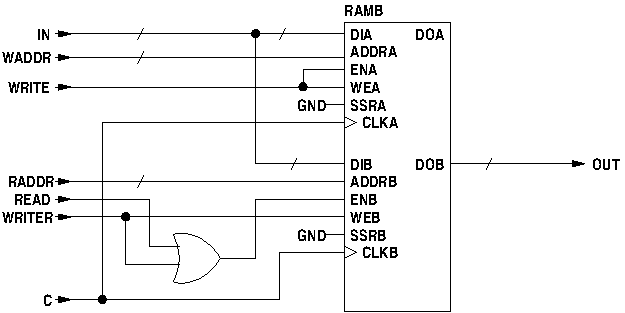
\includegraphics{qbram}

        To make an equivalent functional unit using CLB RAM
        the logic is -

        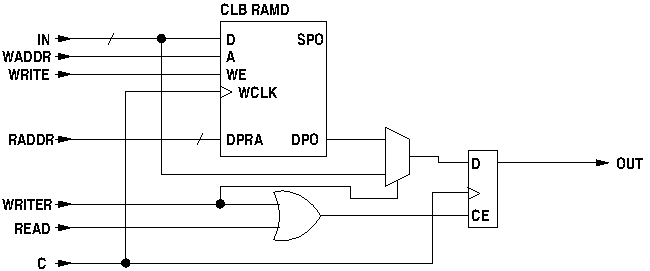
\includegraphics{qcram}

        In both the above blocks {\bf WRITER} writes directly to the
        output register whereas {\bf WRITE} writes to the RAM. {\bf
        READ} reads from the RAM to the output register.

        The code for the memory logic is contained in method
        queuemem() -
        \begin{lstlisting}[gobble=8, language=java]
            private Net[] queuemem (
                int     depth,  // buffer depth
                int     dwidth, // data width
                int     awidth, // address width
                Net[]   in,     // data input
                Net[]   raddr,  // read address
                Net[]   waddr,  // write address
                Net     read,   // read enable
                Net     write,  // write enable
                Net     writer, // write enable for the read port or null
                Net     ci,     // write clock
                Net     co      // read clock
            ) {
                Net[]   out;
                boolean is_sync = (ci == co);

                if (depth <= queue_buffer_max_cram_depth) {
                    // use CLB RAM
                    Net[] o = new Net[dwidth];
                    for (int i=0 ; i<dwidth ; i++)
                        o[i] = new Net("o" + i + "_");
                    sram2(  dwidth,
                              ci, write, waddr,   in, null,
                            null,  null, raddr, null,    o,
                            null, null );
                    if (is_sync)
                        out = reg(mux2(writer, o, in), co, read, null, null, null);
                    else
                        out = reg(o, co, read, null, null, null);
                    return(out);
                }

                // use block RAM
                out = new Net[dwidth];
                for (int i=0 ; i<dwidth ; i++)
                    out[i] = new Net("out" + i + "_");
                Net[]   rin = is_sync ? in : null;
                rram2 ( dwidth, awidth,
                        write,  write, ci, waddr,  in, null,
                         read, writer, co, raddr, rin,  out,
                        null, new ArrayList() );
                return(out);
            }
        \end{lstlisting}

        If the buffer depth is less than or equal to the maximum CLB RAM
        depth (TDECode.queue\_buffer\_max\_cram\_depth) then CLB RAM is
        used (method XFunctions.sram2()), otherwise block RAM is used
        (method XFunctions.rram2()). In the case of a synchronous buffer
        the first write to an empty FIFO asserts {\bf writer} which 
        casues the output register to be directly loaded with the datum.


        The following terms are used in the logic description -

        \blist
        \item   empty - the RAM is empty
        \item   full - the RAM is full
        \item   NE - data is available at the output of the queue buffer
        \item   NF - data can be written to the queue buffer
        \item   read - read RAM
        \item   write - write RAM
        \item   writer - first write when queue buffer empty
        \item   raddr - RAM read address
        \item   waddr - RAM write address
        \item   fcnt - RAM occupancy counter
        \item   $\Uparrow$ - increment
        \item   $\Downarrow$ - decrement
        \blend

        Note that a RAM occupancy counter, {\bf fcnt}, is kept in
        addition to read and write address counters. {\bf fcnt} is
        used to determine the RAM full and empty conditions and is
        potentially faster than doing comparisons between {\bf
        raddr} and {\bf waddr}. Additional counters are used for the
        optional word count and space count, again trading speed for
        logic and routing resources.

        The following table shows the change of state and counter
        increment/decrement operations in controlling the queue
        buffer ({\bf full} and {\bf NF} are not shown) -

        \sf{\small{
        \begin{tabular}{ | c | c | c | c || c | c | c | c | c | c | c |}
        \hline
        \multicolumn{2}{| c |}{state} &
        \multicolumn{2}{ c ||}{inputs} &
        \multicolumn{3}{ c |}{increment/decrement} &
        \multicolumn{3}{ c |}{memory control} &
        new \\
        \cline{1-10}
        empty & NE & PUSH & POP & waddr & raddr & fcnt & write & writer & read & NE\\
        \hline
        1 & 0 & 1 & 0 &            &            &              & 0 & 1 & 0 & 1 \\                     
        0 & 1 & 1 & 0 & $\Uparrow$ &            & $\Uparrow$   & 1 & 0 & 0 & 1 \\           
        1 & 1 & 1 & 0 & $\Uparrow$ &            & $\Uparrow$   & 1 & 0 & 0 & 1 \\           
        0 & 1 & 1 & 1 & $\Uparrow$ & $\Uparrow$ &              & 1 & 0 & 1 & 1 \\           
        1 & 1 & 1 & 1 &            &            &              & 0 & 1 & 0 & 1 \\                     
        0 & 1 & 0 & 1 &            & $\Uparrow$ & $\Downarrow$ & 0 & 0 & 1 & 1 \\       
        1 & 1 & 0 & 1 &            &            &              & 0 & 0 & 0 & 0 \\                    
        \hline
        \end{tabular}
        }}

        On first write to an empty queue buffer the datum is
        written directly to the read port of the RAM block and
        {\bf NE} goes high, but {\bf fcnt} stays at 0 as nothing is
        written to the RAM. The next write (if there is no read) will
        write to RAM and increment both{\bf fcnt} and {\bf waddr}. On
        acknowledging the output datum (i.e. popping a datum off
        the queue) if there is only the datum in the read port register
        {\bf NE} will go low since {\bf fcnt} is 0 ({\bf empty}
        will be true). If there is a datum in the output register and
        another in the RAM then the last RAM read to the port register
        will occur and {\bf fcnt} will decrement from 1 to 0 and
        empty will become true, but NE will not go low until the next
        {\bf POP}.

        Related equations -

        % NF = !full
        % read = POP & !empty
        % write = PUSH & NE & !(empty & POP)
        % writer = PUSH & empty & !(NE & !POP)                  
        $
        \mathsf{NF = \overline{full}} \\
        \mathsf{read = POP \cdot \overline{empty}} \\
        \mathsf{write = PUSH \cdot NE \cdot \overline{(empty \cdot POP)}} \\
        \mathsf{writer = PUSH \cdot empty \cdot \overline{(NE \cdot \overline{POP})}}
        $

        State changes -

        % NE <- !(empty & NE & !PUSH & POP)
        % empty <- !write & (fcnt==0 | fcnt==1 && read)
        % full <- !read & (fcnt==11...11 | fcnt==11...10 & write)
        $
        \mathsf{NE \Leftarrow \overline{empty \cdot NE \cdot \overline{PUSH} \cdot POP}} \\
        \mathsf{empty \Leftarrow \overline{write} \cdot (fcnt==0 + fcnt==1 \cdot read)} \\
        \mathsf{full \Leftarrow \overline{read} \cdot (fcnt==11\cdots11 + fcnt==11\cdots10 \cdot write)}
        $

        Increment/decrement counters -

        % raddr++ = read
        % waddr++ = write
        % fcnt++ = write & !read
        % fcnt-- = read & !write
        $
        \mathsf{raddr\Uparrow = read} \\
        \mathsf{waddr\Uparrow = write} \\
        \mathsf{fcnt\Uparrow = write \cdot \overline{read}} \\
        \mathsf{fcnt\Downarrow = read \cdot \overline{write}}
        $

        The code is -
        \begin{lstlisting}[gobble=8, language=java]
            public Net[] sync_buffer (
                Net[]   in,     // data input
                Net     push,   // write-to-queue input
                Net     pop,    // pop-from-queue input
                Net     c,      // clock
                Net     ne,     // returned not empty
                Net     nf,     // returned not full
                Net[]   count,  // returned buffer data count or null
                Net[]   free,   // returned free space count or null
                Net     r,      // buffer reset
                Net     rr,     // buffer reset output
                boolean fifo,   // use FIFO hardware if present
                int     depth,  // buffer depth - a power of 2 constrained by FPGA family
                Var     wcvar,  // write clock variable
                Var     rcvar   // read clock variable
            ) {
                int     dwidth = in.length;
                Net     empty = new Net("EMPTY");
                Net     full = new Net("FULL");

                if (((this instanceof XC5V) || (this instanceof XC6V)) && (depth >= 512) && (depth <= 8192) && fifo) {
                    // For Virtex5 or Virtex6 block RAM FIFO can use inbuilt FIFO logic.
                    if (rr != null) {
                        if (r != null)
                            rr.connect(r);
                        else
                            rr.connect(Net.LO);
                    }
                    ne.connect(INV(empty));
                    nf.connect(INV(full));
                    Net[]   out = new Net[dwidth];
                    for (int i=0 ; i<dwidth ; i++)
                        out[i] = new Net("out" + i + "_");
                    queuefifo(depth, in, push, pop, out, empty, full, count, free, r, c, c, wcvar, rcvar);
                    return(out);
                }

                int     awidth = bits(depth-1, false);
                Net     read = new Net("READ");
                Net     write = new Net("WRITE");
                Net     writer;
                Net[]   raddr, waddr, out;

                read.connect(AND(pop, INV(empty)));
                write.connect(AND(push, ne, INV(AND(empty, pop))));
                writer = AND(push, empty, INV(AND(ne, INV(pop))));
                ne.connect(FDRS(INV(AND(empty, ne, INV(push), pop)), c, OR(push, pop), r, null, null, null));
                nf.connect(INV(full));

                raddr = cb(awidth, false, c,  read, r, null, null);
                waddr = cb(awidth, false, c, write, r, null, null);

                int     cwidth = awidth + 1;
                Net[]   fcnt;
                Net     ed;
                Net     fd;

                fcnt = cb(awidth, false, c, XOR(read, write), r, read, null);

                ed = AND(INV(write), eqzeros(fcnt, 1, awidth-1), OR(INV(fcnt[0]), read));
                empty.connect(FDRS(ed, c, null, null, r, "S", null));
                fd = AND(INV(read), eqones(fcnt, 1, awidth-1), OR(fcnt[0], write));
                full.connect(FDRS(fd, c, null, r, null, null, null));

                if (count != null) {
                    Net[]   fcntr;
                    fcntr = cb(cwidth, false, c, XOR(pop, push), r, pop, null);
                    connect(count, fcntr);
                }
                if (free != null) {
                    Net[]   ecntr;
                    String  sinit = Integer.toHexString(1 << awidth);
                    ecntr = cb(cwidth, false, c, XOR(pop, push), r, push, sinit);
                    connect(free, ecntr);
                }

                Net mread = OR(read, writer);
                out = queuemem(depth, dwidth, awidth, in, raddr, waddr, mread, write, writer, c, c);
                if (rr != null) {
                    if (r != null)
                        rr.connect(r);
                    else
                        rr.connect(Net.LO);
                }
                return(out);
            }
        \end{lstlisting}
        Calls to constructor Net(), e.g. Net("EMPTY"), create nets which
        have unique identifiers constructed by appending an integer to
        the argument string. The head strings are chosen to label nets
        with meaningful identifiers in the netlist but have no other
        significance.

        If the FPGA is Virtex5 or Virtex6 and the buffer depth is
        between 512 and 8192 inclusive then method queuefifo() is called
        to use the inbuilt block RAM FIFO logic. This can be used for
        both synchronous and asynchronous buffers. The code for this
        method is -
        \begin{lstlisting}[gobble=8, language=java]
            private void queuefifo(
                int     depth,  // buffer depth
                Net[]   in,     // data input
                Net     push,   // true to push a datum
                Net     pop,    // true to pop a datum
                Net[]   out,    // data output
                Net     empty,  // true if the FIFO is empty
                Net     full,   // true if the FIFO is full
                Net[]   count,  // number of contained data
                Net[]   free,   // number of free spaces
                Net     r,      // reset signal or null
                Net     cw,     // write clock
                Net     cr,     // read clock
                Var     wcvar,  // write clock variable
                Var     rcvar   // read clock variable
            ) {
                int     dwidth = in.length;
                int     awidth = bits(depth-1, false);
                Net[]   rdcount = null;
                Net[]   wrcount = null;
                Net         r3 = new Net();
                double      minfreq = Math.min(wcvar.getClkMinFreq(), rcvar.getClkMinFreq());
                double      wcmaxfreq = wcvar.getClkFreq();
                int         rcycles = (int)(Math.ceil(wcmaxfreq / minfreq)) * 4;
                Net[]       srl16in = new Net[1];
                Net[]       srl16out = null;
                ArrayList   srl16init = new ArrayList();
                srl16in[0] = r3;

                for (int i=0 ; i<rcycles ; i++)
                    srl16init.add("1");
                srl16init.add("0");

                if (r != null)
                    srl16out = del(rcycles+1, srl16in, null, cw, OR(r, r3), null, srl16init);
                else
                    srl16out = del(rcycles+1, srl16in, null, cw, r, null, srl16init);
                srl16out[0].connect(r3);

                if (awidth < 9) // should have a variable for this
                    awidth = 9; // minimum block RAM address width (depth 512)

                int bdwidth = ramb_dwidths[awidth];
                int nb = (dwidth - 1) / bdwidth + 1;
                int totwidth = nb * bdwidth;

                if ((count != null) || (free != null)) {
                    rdcount = netArray(awidth);
                    wrcount = netArray(awidth);
                }

                for (int i=0 ; i<nb ; i++) {
                    int l = i * bdwidth;
                    int u = l + bdwidth - 1;
                    if (u >= dwidth)
                        u = dwidth - 1;
                    Net[]   id = (in != null) ? subarray(in, l, u) : null;
                    Net[]   od = (out != null) ? subarray(out, l, u) : null;

                    if (i == 0)
                        FIFO(   depth, id, push, pop, od, empty, full, rdcount, wrcount,
                                r3, cw, cr  );
                    else
                        FIFO(   depth, id, push, pop, od, null, null, null, null,
                                r3, cw, cr  );
                }

                // count and free only used for synchronous queues
                if (count != null) {
                    Net[] xx = sub(wrcount, rdcount, null, false, false);
                    for (int i=0 ; i<(count.length-1) ; i++)
                        count[i].connect(xx[i]);
                    count[count.length-1].connect(full);
                }
                if (free != null) {
                    Net[] yy = sub(rdcount, wrcount, null, false, false);
                    for (int i=0 ; i<(free.length-1) ; i++)
                        free[i].connect(yy[i]);
                    free[free.length-1].connect(full);
                }
            }
        \end{lstlisting}

        Net {\bf r3} is the FIFO reset. This must be high for at least 3
        clock cycles of both the read and the write clock. A reset must
        be done after power-up so is done after configuration. {\bf
        rcycles} is the number of cycles of the write clock {\bf cw}
        necessary for at least 3 cycles of both clocks. The reset pulse
        is generated using one or more CLB shift registers. The initial
        condition is 01...1, so the output is initially 1. The output is
        connected to the CE and the data input so the contents will
        shift until the 0 is at the output at which point it will stop.
        The external reset {\bf r} is ORed in to the CE to start the
        shift sequence of {\bf rcycles} 1s and a 0 each time.

    \subsubsection{async\_buffer()}

        For an asynchronous queue buffer the input and output clocks
        differ and the scheme for avoiding an initial read on a
        write to an empty queue buffer cannot be used. The point at
        which a queue becomes available after a write to an empty
        buffer is now undefined since the clocks are separate and
        unrelated.

        The CLB RAM block now simply has a register on the output
        of the read-only port.

        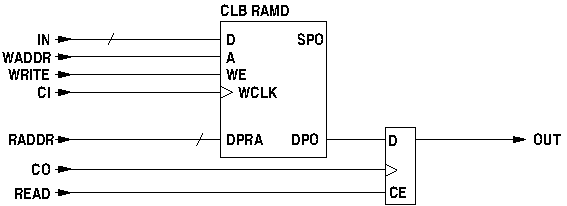
\includegraphics{aqcram}

        The block RAM has no additional logic.

        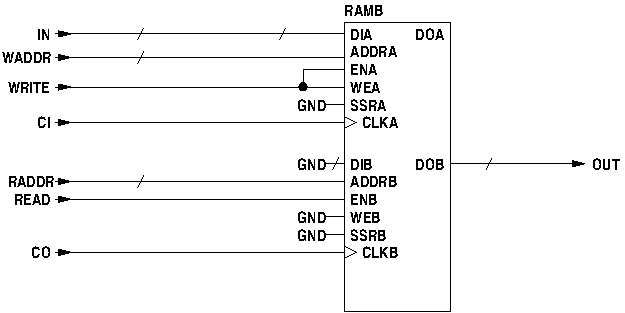
\includegraphics{aqbram}

        In method {\bf queuemem()} described previously the boolean {\bf
        is\_sync} selects whether this extra logic is inserted or not.

        The asynchronous queue buffer uses one of the above RAMs (the
        former for depth 16, the latter for greater depths) and an
        address generator block. The use of address comparison for
        full and empty determination means that the depth of the RAM
        FIFO is $2^n - 1$ however an additional datum is held in the
        RAM output register giving a total buffer depth of $2^n$.
        The additional logic shown provides the first read following
        a write to an empty buffer after which {\bf NE} is raised.

        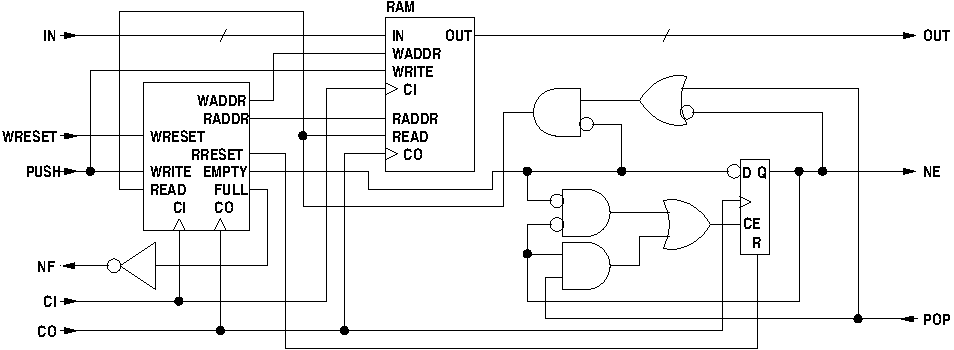
\includegraphics{asyncqueuebuffer}

        The code for this is -
        \begin{lstlisting}[gobble=8, language=java]
            public Net[] async_buffer (
                Net[]   in,     // the data input
                Net     push,   // push-to-queue input
                Net     pop,    // pop-from-queue input
                Net     ci,     // input clock
                Net     co,     // output clock
                Net     ne,     // returned not empty
                Net     nf,     // returned not full
                Net[]   wstat,  // returned status synchronised to the read clock
                Net[]   rstat,  // returned status synchronised to the write clock
                Net     r,      // reset input synchronised to the write clock or null
                Net     rr,     // reset output synchronised to the read clock or null
                boolean fifo,   // use FIFO hardware if present
                int     depth,  // buffer depth
                Var     wcvar,  // write clock variable
                Var     rcvar   // read clock variable
            ) {
                Net     full = new Net("FULL");
                Net     empty = new Net("EMPTY");
                int     dwidth = in.length;

                if (((this instanceof XC5V) || (this instanceof XC6V)) && (depth >= 512) && (depth <= 8192) &&
                    (wstat == null) && (rstat == null) && fifo) {
                    // For Virtex5 or Virtex6 block RAM FIFO can use inbuilt FIFO logic.
                    if (rr != null) {
                        if (r != null)
                            rr.connect(r);
                        else
                            rr.connect(Net.LO);
                    }
                    ne.connect(INV(empty));
                    nf.connect(INV(full));
                    Net[]   out = new Net[dwidth];
                    for (int i=0 ; i<dwidth ; i++)
                        out[i] = new Net("out" + i + "_");
                    queuefifo(depth, in, push, pop, out, empty, full, null, null, r, ci, co, wcvar, rcvar);
                    return(out);
                }

                int     awidth = bits(depth-1, false);
                Net[]   waddr = new Net[awidth];
                Net[]   raddr = new Net[awidth];
                Net     read;
                Net     write = push;
                Net[]   out;
                Net     oack;

                if ((rr == null) && (r != null))
                    rr = new Net("rr");

                nf.connect(INV(full));

                for (int i=0 ; i<awidth ; i++) {
                    waddr[i] = new Net("WADDR" + i + "_");
                    raddr[i] = new Net("RADDR" + i + "_");
                }

                oack = OR(AND(ne, pop), AND(INV(ne), INV(empty)));

                asynch_fifo_control (
                    write, ne, pop, ci, co, r,                      // input nets
                    waddr, raddr, rstat, wstat, full, empty, rr,    // output nets
                    awidth, depth
                );

                ne.connect(FDRS(INV(empty), co, oack, rr, null, null, null));

                read = AND(OR(INV(ne), pop), INV(empty));
                out = queuemem(depth, dwidth, awidth, in, raddr, waddr, read, write, null, ci, co);
                return(out);
            }
        \end{lstlisting}

        If the FPGA is Virtex5 or Virtex6 and the buffer depth is
        between 512 and 8192 inclusive and the write status ({\bf
        wstat}) and read status arguments ({\bf rstat}) are null and
        parameter {\bf fifo} is true then method {\bf queuefifo()} is
        called to use the FIFO logic associated with block RAMs (the
        read and write status cannot be derived from that logic).

        As in the schematic diagram above the two main blocks are
        memory (method {\bf queuemem()}) and asynchronous control
        logic (method {\bf asynch\_fifo\_control()}).


        Resetting an asynchronous queue buffer must be carried out with
        care. A pending read must be allowed to complete after which
        {\bf NE} will go low and no more reads will occur (since the
        queue buffer is now empty). A pending write must be ignored and
        {\bf NF} forced low (the source will now remove {\bf PUSH},
        withdrawing the write request). {\bf NF} must remain low during
        the reset process (which may be many cycles if the input clock
        is higher than the output clock) and then go high when the now
        empty queue buffer is again available for writing.

        The reset input is synchronised to the write (input) clock.
        When asserted it resets the write address and clears the
        full flip-flop (and holds it clear during the reset
        process). At the same time it sets a blocking flip-flop to
        force {\bf NF} low so that a write will not occur (the reset
        also immediately forces {\bf NF} low to supress a possible
        write in the current cycle). The reset is resynchronised to
        the read (output) clock to later reset the read address, the
        empty flip-flop and the {\bf NE} flag. A further pulse is
        then generated once again in the input clock domain to
        finally free the blocking flip-flop and raise {\bf NF} after
        the output side has been reset. This mechanism is necessary
        to avoid attempts to write to the buffer before the output
        side is reset. On the other hand the output side reset must
        be synchronised to the output clock so that it can fit in
        with pending reads, lowering {\bf NE} synchronously with the
        output to stop further reads.

        If the queue buffer is never reset the reset logic
        is omitted.

        The address generator follows the design given in Xilinx
        application note 131.

        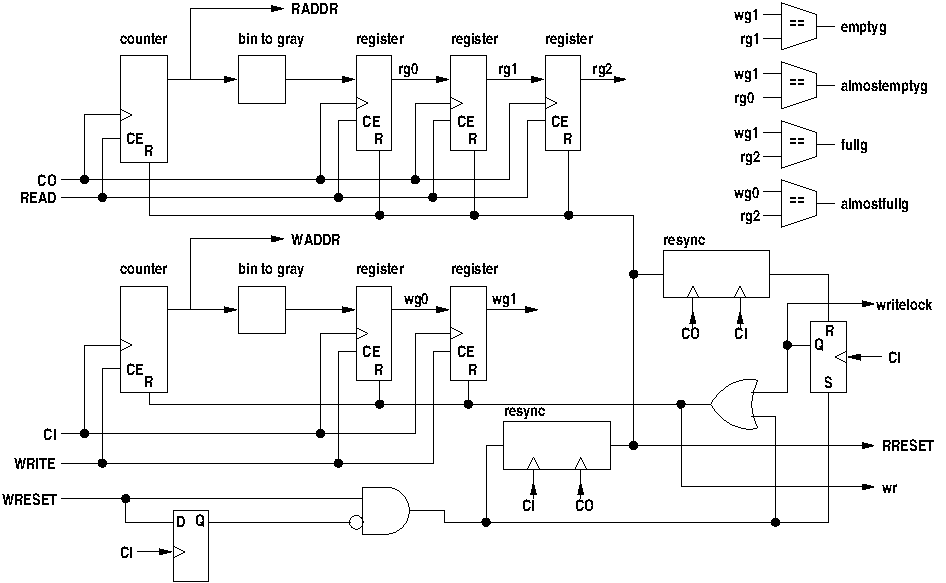
\includegraphics{asyncaddr}

        When {\bf WRESET} is asserted it resets the write address
        counter to zero and the following grey code registers
        to the initial values -

        \begin{tabular}{c c}
        wg0 & 100...000 \\
        wg1 & 100...001 \\
        \end{tabular}

        At the same time it is gated through to {\bf FULL} and
        also latched in a flip-flop so that
        the queuebuffer appears full and will not be written on the
        current or subsequent clock cycles. The write reset is
        resynchronised to the read clock and the resulting signal
        is output to {\bf RRESET} for possible daisy chaining to
        further queues in the pipeline. {\bf RRESET} also resets the
        {\bf EMPTY} flip-flop,
        resets the read address counter to zero and the following
        grey code registers to the initial values -

        \begin{tabular}{c c}
        rg0 & 100...000 \\
        rg1 & 100...001 \\
        rg2 & 100...011 \\
        \end{tabular}

        These initial values on the write and read sides ensure the queue
        buffer appears initially empty and empty after a reset. The
        values are the gray code sequence leading up to the current read
        and write addresses of 0 (gray code 0) and hence are gray code
        equivalents of -1, -2 and -3.

        {\bf RRESET} is then resynchronised back to the write
        clock and resets the flip-flop holding {\bf FULL} asserted.
        The reset process thus takes a number of read and write
        clock cycles, the exact duration depending on the two clock
        frequencies. The reset inhibits any writes on the current
        clock cycle and from then on until the reset is complete.
        The queue buffer does not appear empty immediately the
        reset is asserted on the write side, however only one read
        can take place (if the queue buffer is not already empty) and
        that will read a correct datum. After that the queue buffer
        will be reset on the read side and will appear empty. The
        queue buffer can then only appear non-empty after a
        subsequent write following the reset.

        The gray code address comparisons at various phases are
        compared to determine empty and full conditions -

        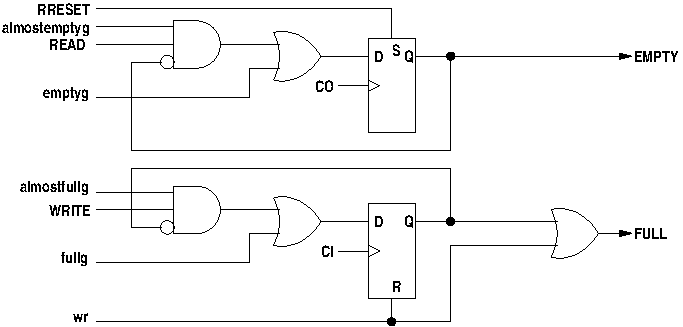
\includegraphics{asyncfullempty}

        The binary to gray code converter logic is -

        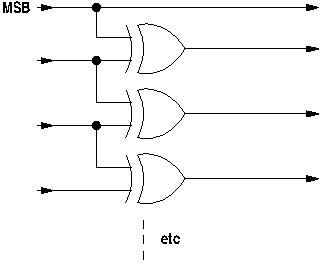
\includegraphics{bintogray}

        which is coded as -
        \begin{lstlisting}[gobble=8, language=java]
            private Net[] bin_to_gray (Net[] in) {
                int     size = in.length;
                Net[]   out = new Net[size];

                out[size-1] = in[size-1];
                for (int i=size-2 ; i>=0 ; i--)
                    out[i] = XOR(in[i+1], in[i]);
                return(out);
        }
        \end{lstlisting}

        The asynchronous control logic in method
        asynch\_fifo\_control() is coded as -
        \begin{lstlisting}[gobble=8, language=java]
            private void asynch_fifo_control (
                Net write, Net ne, Net pop, Net wc, Net rc, Net r,      // input nets
                Net[] waddr, Net[] raddr,                               // output nets
                Net[] rstat, Net[] wstat, Net full, Net empty, Net rr,  // output nets
                int awidth, int depth
                // write is the write enable
                // ne is true if the asynchronous FIFO is not empty
                // pop is true to pop a datum
                // wc is the write clock
                // rc is the read clock
                // r is a reset synchronised to the write clock or null
                // waddr is the write address
                // raddr is the read address     
                // rstat is the read buffer status
                // wstat is the write buffer status
                // full is the net to return the full condition
                // empty is the net to return the empty condition
                // rr is a reset synchronised to the read clock
                // awidth is the address width
                // depth is the FIFO depth
            ) {
                Net[]   wg0, wg1, rg0, rg1, rg2;
                Net     emptyg, almostemptyg, fullg, almostfullg;
                Net     wr = null;  // extended write reset
                Net     writelock = null;
                Net     read;
                // Initial gray code values of pipelined read and write address registers.
                // These are address sequences leading up to the initial read and
                // write addresses of 0, hence they are gray code values of -1, -2 and -3.
                String  igm1 = intToGrayString(-1, awidth);
                String  igm2 = intToGrayString(-2, awidth);
                String  igm3 = intToGrayString(-3, awidth);

                if ((r != null) && r.isConnected(Net.LO))
                    r = null;
                if (r != null) {
                    r = AND(r, INV(FDRS(r, wc, null, null, null, null, null)));
                    rr.connect(resync(r, wc, rc));
                    writelock = FDRS(null, wc, null, resync(rr, rc, wc), r, "R", null);
                    wr = OR(r, writelock);
                } else if (rr != null)
                    rr.connect(Net.LO);

                read = AND(OR(INV(ne), pop), INV(empty));

                connect(raddr, cb(awidth, false, rc, read, rr, null, null));
                rg0 = reg(bin_to_gray(raddr), rc, read, rr, igm1, null);
                rg1 = reg(rg0, rc, read, rr, igm2, null);
                rg2 = reg(rg1, rc, read, rr, igm3, null);

                connect(waddr, cb(awidth, false, wc, write, wr, null, null));
                wg0 = reg(bin_to_gray(waddr), wc, write, wr, igm1, null);
                wg1 = reg(wg0, wc, write, wr, igm2, null);

                emptyg       = eq(wg1, rg1, false, false);
                almostemptyg = eq(wg1, rg0, false, false);
                fullg        = eq(wg1, rg2, false, false);
                almostfullg  = eq(wg0, rg2, false, false);
                Net empty_d;
                if (lutwidth >= 5)
                    empty_d = OR(AND(OR(INV(ne), pop), INV(empty), almostemptyg), emptyg);
                else {
                    Net n = AND(OR(INV(ne), pop), INV(empty), almostemptyg);
                    empty_d = MUXF5(emptyg, n, Net.HI);
                }
                empty.connect(FDRS(empty_d, rc,  null, null, rr, "S", null));
                if (r != null) {
                    Net full_;
                    full_ = FDRS(OR(fullg, AND(almostfullg, write, INV(full))), wc, null, wr, null, "R", null);
                    full.connect(OR(full_, wr));
                } else
                    full.connect(FDRS(OR(fullg, AND(almostfullg, write, INV(full))), wc, null, null, null, "R", null));

                if ((rstat != null) || (wstat != null)) {
                    Net[]   rgtop, wgtop;
                    rgtop = new Net[2];
                    wgtop = new Net[2];
                    rgtop[0] = rg1[awidth-2];
                    rgtop[1] = rg1[awidth-1];
                    wgtop[0] = wg1[awidth-2];
                    wgtop[1] = wg1[awidth-1];
                    if (rstat != null)
                        asynch_fifo_control_status(rstat, rgtop, wgtop, rc, rr);
                    if (wstat != null)
                        asynch_fifo_control_status(wstat, rgtop, wgtop, wc, wr);
                }
            }
        \end{lstlisting}

        Method {\bf asynch\_fifo\_control\_status()}, which is called if
        the read status ({\bf rstat}) or write status ({\bf wstat})
        arguments are non-null, generates logic to return the buffer
        occupancy status. This status gives an approximate view, the
        asynchronous nature of the queue buffer precluding actual
        occupancy counts.

        \begin{lstlisting}[gobble=8, language=java]
            private void asynch_fifo_control_status (Net[] stat, Net[] rgtop, Net[] wgtop, Net c, Net r) {
                Net n, n1, n2, n3, n4;
                // Empty to 1/4 Full - quads equal
                n = AND(eq(rgtop, wgtop, false, false), INV(OR(stat[3], stat[4])));
                stat[0].connect(FDRS(n, c,  null, null, r, "S", null));
                // 1 word to 1/2 Full - quad 1 ahead
                n1 = AND(decode(rgtop, 0), decode(wgtop, 1));
                n2 = AND(decode(rgtop, 1), decode(wgtop, 3));
                n3 = AND(decode(rgtop, 3), decode(wgtop, 2));
                n4 = AND(decode(rgtop, 2), decode(wgtop, 0));
                n = OR(n1, n2, n3, n4);
                stat[1].connect(FDRS(n, c, null, r, null, "R", null));
                // 1/4 full to 3/4 Full - quad 2 ahead
                n1 = AND(decode(rgtop, 0), decode(wgtop, 3));
                n2 = AND(decode(rgtop, 1), decode(wgtop, 2));
                n3 = AND(decode(rgtop, 3), decode(wgtop, 0));
                n4 = AND(decode(rgtop, 2), decode(wgtop, 1));
                n = OR(n1, n2, n3, n4);
                stat[2].connect(FDRS(n, c, null, r, null, "R", null));
                // 1/2 Full to Full - quad 3 ahead
                n1 = AND(decode(rgtop, 0), decode(wgtop, 2));
                n2 = AND(decode(rgtop, 1), decode(wgtop, 0));
                n3 = AND(decode(rgtop, 3), decode(wgtop, 1));
                n4 = AND(decode(rgtop, 2), decode(wgtop, 3));
                n = OR(n1, n2, n3, n4);
                stat[3].connect(FDRS(n, c, null, r, null, "R", null));
                // 3/4 Full to Full - quad 4 ahead/equal
                n = AND(eq(rgtop, wgtop, false, false), OR(stat[3], stat[4]));
                stat[4].connect(FDRS(n, c, null, r, null, "R", null));
            }
        \end{lstlisting}




    \subsubsection{triggerbuffer()}

        This method creates a synchronous or asynchronous queue buffer
        that has only the control logic and no actual data buffer.
        The code is just the control logic taken from
        methods {\bf sync\_buffer()} and {\bf async\_buffer()}.


    \subsubsection{queueunbuffered()}
    
        A synchronous unbuffered queue is not really a queue and hence
        the control inputs and outputs are labelled differently to
        a buffered queue -
        
        \begin{tabular}{l l}
        buffered & unbuffered\\
        \\
         NE     & ravail  \\
         NF     & wavail  \\
         PUSH   & wpending\\
         POP    & rpending\\
        \end{tabular}

        A synchronous unbuffered queue is created by connecting the {\bf ravail}
        output net to the {\bf wpending} input net and the {\bf wavail} output
        net to the {\bf rpending} input net. With these cross connections
        asserting the {\bf wpending} input asserts the {\bf ravail} output and
        the queue now has read availability. In the same way asserting the {\bf
        rpending} input asserts the {\bf wavail} output and the queue now
        exhibits write availability. These cross connections are valid because
        wpending implies a write is ready to proceed and that a read can now be
        made. Similarly rpending implies that  read is ready to proceed and
        hence a write can now be executed. The rpending and wpending logic
        cannot be driven from the {\bf START\_DEL} output of two EXECPs as for a
        buffered queue as these are not asserted until the availability outputs
        are asserted. This circular logic will deadlock. Instead the {\bf
        wpending} and {\bf rpending} inputs are driven by the {\bf PENDING}
        output of EXECPs. This has been described previously (\ref{ubqueuerw}). The data
        output is simply connected to the data input as the unbuffered queue
        does not store anything.

        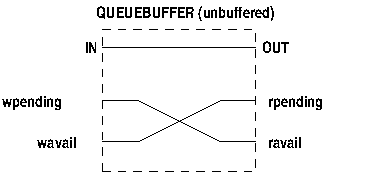
\includegraphics{ubqueue}

        \begin{lstlisting}[gobble=8, language=java]
            ravail.connect(wpending);
            wavail.connect(rpending);
            return(in);
        \end{lstlisting}

        Asynchronous unbuffered queues are not implemented.



    \subsubsection{queuefifo()}
    
        For synchronous queues created by {\bf sync\_buffer()} or asynchronous
        queues created by {\bf async\_buffer()}, if the FPGA is Virtex 5, Virtex 6
        or system7 and the depth is less than 8192 and the fifo attribute has been
        set on the queue, then methid {\bf queuefifo()} will be called. This will in
        turn call {\bf fifallocate()} in the FPGA class. This in turn will
        construct a list of {\bf FifoBlock} instances to the required width and
        then call method FIFO() in class {\bf FifoBlock} on each to construct the
        block RAM FIFOs.



\subsection{delay line}

    \begin{lstlisting}[gobble=4, language=java]
        public Net[] del (
            int         n,      // line length
            Net[]       in,     // input net array
            Net[]       len,    // optional variable length selection input
            Net         c,      // clock
            Net         ce,     // optional clock enable
            Net         r,      // optional reset
            ArrayList   init    // initial delay line contents as a list of
                                // hexadecimal strings
        ) {
            if ((n == 0) && (len == null))
                return(in);

            int             blklen = 1 << srladdrwidth;
            int             width = in.length;
            Net[]           out = new Net[width];
            boolean         flip_flops = (n == 1) || ((r != null) && (!r.isConnected(Net.LO)));
            boolean         varlen = (len != null);
            StringBuffer    binit = null;
            int             del_len;

            if (varlen)
                n = blklen;

            for (int k=0 ; k<width ; k++) {
                // if delay of only 1 use flip-flop
                // if reset input is used, must use flip-flops
                if (flip_flops) {
                    Net[]   s = new Net[n+1];
                    s[0] = in[k];
                    for (int i=0 ; i<n ; i++)
                        if ((init == null) || strhexbit((String)init.get(i), k) == 0)
                            s[i+1] = FDRS(s[i], c, ce, r, null, "R", null);
                        else
                            s[i+1] = FDRS(s[i], c, ce, null, r, "S", null);
                    out[k] = s[n];
                    continue;
                }

                // use delay lines
                String sinit;
                if (init != null) {
                    binit = new StringBuffer();
                    for (int i=0 ; i<n ; i++) {
                        int b = strhexbit((String)init.get(i), k);
                        binit.insert(0, (b == 0) ? "0" : "1");
                    }
                    sinit = binToHex(binit);
                } else
                    sinit = "0";
                if (varlen) {
                    // variable length
                    switch (srladdrwidth) {
                    case 4:
                        out[k] = SRL16E(in[k], c, ce, len, sinit, null);
                        break;
                    case 5:
                        out[k] = SRL32E(in[k], c, ce, len, sinit, false, null);
                    }
                } else {
                    // Constant length.
                    // Insert a flip-flop at the output to improve timing,
                    // so use n-1 as length.
                    int     blocks = (n - 2) / blklen + 1;
                    Net[]   s = new Net[blocks+1];
                    boolean q31;
                    int     ffinit = 0;
                    if ((binit != null) && (binit.charAt(binit.length() - n) == '1')) {
                         // remove 1 bit - used with flip-flop
                        ffinit = 1;
                        binit.deleteCharAt(binit.length() - n);
                    }
                    len = new Net[srladdrwidth];
                    s[0] = in[k];
                    for (int i=0, count=n-1 ; i<blocks ; i++, count-=blklen) {
                        int m = (count < blklen) ? count-1 : blklen-1;
                        for (int j=0 ; j<srladdrwidth ; j++)
                            len[j] = (((m >> j) & 1) == 1) ? Net.HI : Net.LO;
                        if (binit != null)
                            sinit = binToHex(binit);
                        switch (srladdrwidth) {
                        case 4:
                            s[i+1] = SRL16E(s[i], c, ce, len, stringsize(sinit, srladdrwidth), null);
                            break;
                        case 5:
                            q31 = (i != (blocks - 1));
                            s[i+1] = SRL32E(s[i], c, ce, len, stringsize(sinit, srladdrwidth), q31, null);
                        }
                        del_len = 1 << srladdrwidth;
                        if (binit != null) {
                            if (binit.length() >= del_len)
                                binit.delete(binit.length() - del_len, binit.length());
                            else
                                binit.delete(0, binit.length());
                        }
                    }

                    if ((init == null) || ffinit == 0)
                        out[k] = FDRS(s[blocks], c, ce, r, null, "R", null);
                    else
                        out[k] = FDRS(s[blocks], c, ce, null, r, "S", null);
                }
            }
            return(out);
        }
    \end{lstlisting}

    A delay line can be fixed or variable length and may be initialised.
    An initialised delay line with feedback can be used to generate a
    sequence. The parameter {\bf init} is a list of hexadecimal strings,
    one per delay line stage, i.e. each string is a value across the
    width of the delay line.

    Variable {\bf blklen} is the length of an SRL shift register (16 or
    32 depending on FPGA). If the delay line is to have variable length
    ({\bf varlen} is true) it is limited to a maximum of blklen (line
    21).

    Variable {\bf flip\_flops} is true if the delay line length is 1 or if
    the reset {\bf r} is non-null and is not tied false. If true, flip-flops
    will be used to construct the delay line rather than CLB shift registers
    (shift registers cannot be reset).

    The outer loop starting at line 22 takes each bit of the data width
    in turn.

    If {\bf flip\_flops} is true (line 25) flip-flops are used for the
    delay line. The inner loop starting at line 28 iterates along the
    length of the delay line creating an FDRS for each bit. The FDRS is
    initialised by extracting the matching bit from the initialisation
    string and either the {\bf R} or {\bf S} input is connected to net
    {\bf r} as appropriate. On completion of the inner loop the
    continue statement skips to line 98 to continue the outer loop.

    Where shift CLB registers are used ({\bf flip\_flops} is false)
    the initialisation data must be transposed as the SRL registers
    run lengthwise. This is done into variable {\bf sinit}. If the
    shift register is variable length then a single SRL16 or SRL32
    is created. The net array {\bf len} is the address input to select
    the length of the line dynamically.

    If the length of the line is fixed then SRL16 or SRL32 elements are
    concatenated in the loop starting at line 71 to get the required
    line length. The data inputs, data outputs, line length and
    initialisation data are all segmented to match the concatenated
    elements. Note that the final unit of the delay line is implemented
    using flip-flops. This is done because the output-to-clock delay of
    an SRL16 or SRL32 is quite long and this can cause problems with
    timing constraints. The addition of a trailing flip-flop alleviates
    this problem. Note that a variable length line cannot have trailing
    flip-flops (unless a minimum delay of 2 were acceptable) and hence
    may experience timing constraint problems.


\subsection{shifters}

    Left and right fixed shift is performed by methods {\bf lshift()}
    and {\bf rshift()}. These generate no logic and simply connect
    the output net array to the input net array with a displacement.
    Padding to GND is done to outputs shifted off-end except in the
    case of signed most significant bits which are connected to the
    input MSB (sign bit).

    Variable shift is performed by method {\bf var\_shift3pl()}.
    \begin{lstlisting}[gobble=4, language=java]
        public Net[] var_shift3pl (
            Net[]   a,      // input argument - signed or unsigned
            Net[]   s,      // shift argument - unsigned
            int     owidth, // output bit width
            boolean right,  // true for right shift, false for left shift
            boolean signeda // true if the input is signed
        ) {
            int     iwidth = a.length;
            int     shiftsize = s.length;
            int     shiftbits = (1 << shiftsize) - 1;
            long    ssize = Math.min(shiftbits, owidth);
            int     shiftdim = bits(ssize, false);  
            Net[]   shift = new Net[shiftdim];
            int     stages = shiftdim;
            Net[][] v = new Net[stages+1][owidth];
            Net     p1, p2;
            Net[]   o = new Net[owidth];
            int     i, j, k, l, l1, l2;

            if (right) {
                if (signeda)
                    p1 = a[iwidth-1];
                else
                    p1 = Net.LO;
                p2 = Net.LO;

            } else {
                if (signeda)
                    p2 = a[iwidth-1];
                else
                    p2 = Net.LO;
                p1 = Net.LO;
            }

            // prune the shift array to match the output width if too big
            shift = subarray(s, 0, shiftdim-1);

            for (i=0 ; i<iwidth ; i++)
                if (right)
                    // reverse input bit order for right shift
                    v[0][i] = a[iwidth-i-1];
                else
                    v[0][i] = a[i];

            k = iwidth;
            for (j=1 ; j<=stages ; j++) {
                k = Math.min(owidth, iwidth + (1 << j) - 1);
                l = iwidth + (1 << (j-1)) - 1;
                for (i=0 ; i<k ; i++) {
                    l1 = i - (1 << ( j - 1));
                    l2 = i;
                    if (l1 < 0)
                        v[j][i] = mux2(shift[j-1], v[j-1][l2], p1);
                    else if (l2 >= l)
                        v[j][i] = mux2(shift[j-1], p2, v[j-1][l1]);
                    else
                        v[j][i] = mux2(shift[j-1], v[j-1][l2], v[j-1][l1]);
                }
            }

            for (i=0 ; i<owidth ; i++)
                if (right)
                    // reverse output bit order for right shift
                    o[owidth-i-1] = v[stages][i];
                else
                    o[i] = v[stages][i];
            return(o);
        }
    \end{lstlisting}

    This constructs a variable left shift and simply reverses both input
    and output arrays for a right shift. The shift is unsigned so it
    cannot be negative. The shift is accomplished by successive stages
    of multiplexers which select either unshifted bits or bits shifted
    by a power of 2. Each stage is controlled by one bit of the shift
    value. Note that the extra width of the output array (over that of
    the input array) is handled differently depending on whether the
    shift is left or right. The output width is determined in
    constructor nodes.ArgParams() called from nodes.ExprNode.getVal()
    and depends on the input type. For a signed or unsigned integer
    the width is expanded for left shift but not for right shift. Thus
    for right shift the bits shifted off end are lost. For fixed point
    types right shift bits are retained within the fractional part
    of the word but are lost beyond that. Where the output array is
    smaller than the output array of the shifter, {\bf v[stages][]},
    the output array is assigned at the lower subscript end and the
    higher subscript bits are not connected.
    The resulting logic is illustrated by the following diagram
    for the case of 8-bit input and a 3-bit shift value -

    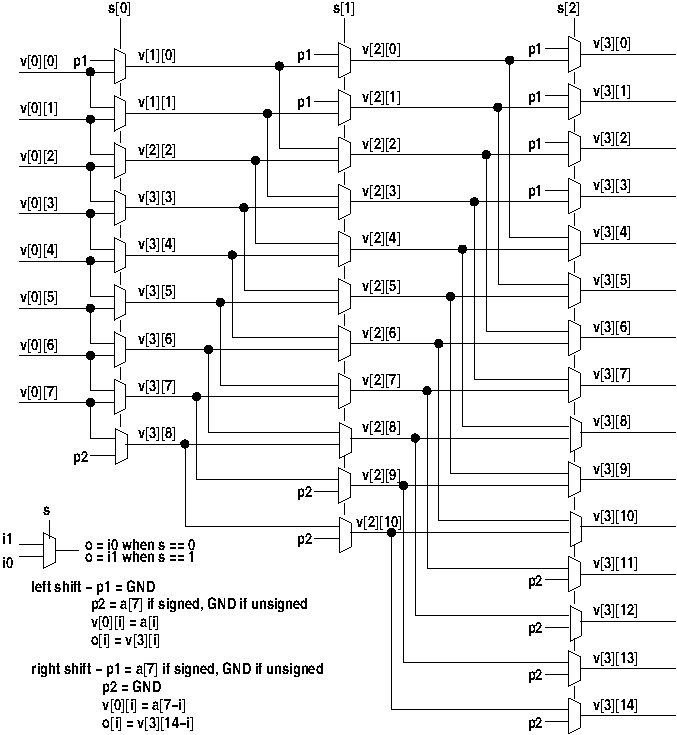
\includegraphics{vshift}


\subsection{adder}


    \begin{lstlisting}[gobble=4, language=java]
        public Net[] add (Net[] a, Net[] b, boolean asigned, boolean bsigned, int osize) {
            int     awid = a.length + ((!asigned && bsigned) ? 1 : 0);
            int     bwid = b.length + ((asigned && !bsigned) ? 1 : 0);
            int     isize = Math.max(awid, bwid);

            if (osize == 0)
                osize = isize + 1;

            Net[]   ps = new Net[osize];    // partial sum
            Net[]   s = new Net[osize];     // sum
            Net[]   c = new Net[osize];     // carries

            a = sig_expand(a, osize, asigned);
            b = sig_expand(b, osize, bsigned);

            int i = 0;

            // Starting at the LSB, while either operand is GND simply copy
            // the other operand to the output. When neither is GND, exit
            // the loop and proceed to normal addition logic for the rest of the
            // bits.
            for ( ; i<osize ; i++) {
                if (a[i].isConnected(Net.LO))
                    s[i] = b[i];
                else if (b[i].isConnected(Net.LO))
                    s[i] = a[i];
                else
                    break;
            }
            if (i < osize)
                c[i] = Net.LO;  // start carry chain if adder still needed

            // Adder stages (if required; i < size).
            int ilast = osize - 1;
            if (!needCPLDarith()) {
                // FPGAs
                for ( ; i<osize ; i++) {
                    if (add_sub_use_lut)
                        ps[i] = LUT("I0^I1", a[i], b[i]);
                    else
                        ps[i] = XOR(a[i], b[i]);
                    s[i] = XORCY(ps[i], c[i]);
                    if (i != ilast)
                        c[i+1] = MUXCY(ps[i], a[i], c[i]);
                }
            } else {
                // CPLDs
                for ( ; i<osize ; i++) {
                    if (cpld_use_lut)
                        s[i] = LUT("I0^I1^I2", a[i], b[i], c[i]);
                    else
                        s[i] = OR(  AND(    a[i],  INV(b[i]), INV(c[i])),
                                    AND(INV(a[i]),     b[i],  INV(c[i])),
                                    AND(INV(a[i]), INV(b[i]),     c[i]),
                                    AND(    a[i],      b[i],      c[i])   );
                    if (i != ilast) {
                        if (cpld_use_lut)
                            c[i+1] = LUT("I0*I1*!I2+I0*!I1*I2+!I0*I1*I2+I0*I1*I2",
                                                                a[i], b[i], c[i]);
                        else
                            c[i+1] = OR(    AND(    a[i],      b[i], INV(c[i])),
                                            AND(    a[i],  INV(b[i]),    c[i]),
                                            AND(INV(a[i]),     b[i],     c[i]),
                                            AND(    a[i],      b[i],     c[i])  );
                    }
                }
            }

            return(s);
        }
    \end{lstlisting}

    This creates an adder. The input nets may be different sizes. The
    output net is one larger than the largest input net. The MSB of
    the result is the final carry bit.

    If the bits of one operand starting from the least significant end
    are a sequence of zeros (GND) then those adder stages are omitted
    and corresponding bits from the other operand become the sum
    bits. The adder stages are constructed from this point onwards
    (note that the for loops do not initialise loop variable {\bf i}
    which remains at the point the input constant search finished).
    If the two operands do not have overlapping variable bits then
    the extra top bit is set appropriately (0 or one of the signs)
    and no adder stages are constructed (i == size so the following
    for loops do not execute).

    For FPGAs the carry chain is used.

    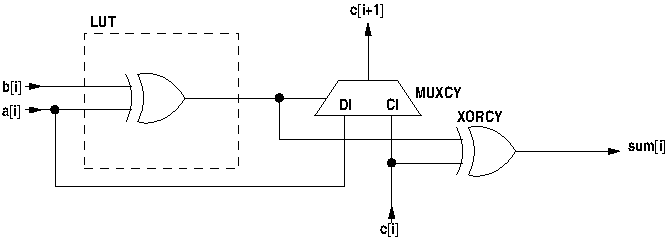
\includegraphics{add}

    If {\bf needCPLDarith()} returns true then the adder is constructed
    only from LUT logic because there is no carry chain available.

    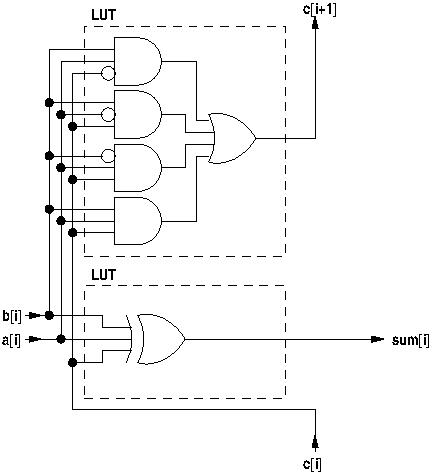
\includegraphics{add_ncc}

    The variables {\bf add\_sub\_use\_lut} and {\bf cpld\_use\_lut} are public
    static variables in ThreePL.jj and select whether the combinatorial
    logic is expressed as a LUT or a combination of AND, OR, XOR and
    INV elements. While the boolean logic is identical the ability of
    the place-and-route tools to optimise the logic may be affected
    by the choice. By default these variables are true to select
    encoding as LUTs. The {\bf -G} option to 3PL renders these
    variables (and many similar ones in other methods) false.



\subsection{inverter}

    The code to create a 1's complement inverter is trivial.


\subsection{incrementer}

    The incrementer method is only used for signed division (method {\bf
    part\_sdiv(})) and for an up/down counter ({\bf method cb()}). It is
    derived from the code for method {\bf add()} with the second input
    {\bf b} omitted and the carry input connected to an {\bf enable}
    input. Thus when {\bf enable} is low the output is the same as the
    input {\bf a} and when {\bf enable} is high the output
    is {\bf a} + 1. The result is the same width as the input, not one
    greater.


\subsection{subtracter}

    \begin{lstlisting}[gobble=4, language=java]
        public Net[] sub (Net[] a, Net[] b, boolean asigned, boolean bsigned, int osize) {
            int     awid = a.length + ((!asigned && bsigned) ? 1 : 0);
            int     bwid = b.length + ((asigned && !bsigned) ? 1 : 0);
            int     isize = Math.max(awid, bwid);

            if (osize == 0)
                osize = isize + 1;

            Net[]   pd = new Net[osize]; // partial difference
            Net[]   d = new Net[osize];  // difference
            Net[]   c = new Net[osize];  // carries

            a = sig_expand(a, osize, asigned);
            b = sig_expand(b, osize, bsigned);

            int i = 0;

            // Starting at the LSB, while 2nd operand is GND simply copy
            // the 1st operand to the output. When 2nd operand is no
            // longer GND, exit the loop and proceed to normal subtraction
            // logic for the rest of the bits. 2nd operand should never be
            // all zeros as the subtraction would have been optimised out
            // prior to this.
            for ( ; i<osize ; i++) {
                if (b[i].isConnected(Net.LO))
                    d[i] = a[i];
                else
                    break;
            }
            c[i] = Net.HI;

            int ilast = osize - 1;
            if (!needCPLDarith()) {
                // FPGAs
                for ( ; i<osize ; i++) {
                    if (add_sub_use_lut)
                        pd[i] = LUT("I0^!I1", a[i], b[i]);
                    else
                        pd[i] = XOR(a[i], INV(b[i]));
                    d[i] = XORCY(pd[i], c[i]);
                    if (i != ilast)
                        c[i+1] = MUXCY(pd[i], a[i], c[i]);
                }
            } else {
                // CPLDs
                for ( ; i<osize ; i++) {
                    if (cpld_use_lut)
                        d[i] = LUT("I0^!I1^I2", a[i], b[i], c[i]);
                    else
                        d[i] = OR(  AND(    a[i],      b[i],   INV(c[i])),
                                    AND(INV(a[i]), INV(b[i]),  INV(c[i])),
                                    AND(INV(a[i]),     b[i],       c[i]),
                                    AND(    a[i],  INV(b[i]),      c[i])   );
                    if (i != ilast)
                        if (cpld_use_lut)
                            c[i+1] = LUT("I0*!I1*!I2+!I0*!I1*I2+I0*I1*I2+I0*!I1*I2",
                                                                a[i], b[i], c[i]);
                        else
                            c[i+1] = OR(    AND(    a[i],  INV(b[i]), INV(c[i])),
                                            AND(    a[i],      b[i],      c[i]),
                                            AND(INV(a[i]), INV(b[i]),     c[i]),
                                            AND(    a[i],  INV(b[i]),     c[i])  );
                }
            }
            return(d);
        }
    \end{lstlisting}

    The input operands are expanded to the size of the largest of the
    two plus one to match the required size of the difference.

    If the bits of the second operand starting from the least
    significant end are a sequence of zeros (GND) then those subtracter
    stages are omitted and corresponding bits from the other operand
    become the difference bits. The subtracter stages are constructed
    from this point onwards (note that the for loops do not initialise
    loop variable {\bf i} which remains at the point the input constant
    search finished).

    For FPGAs the carry chain is used.

    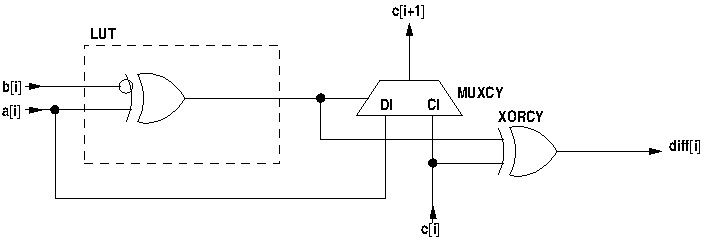
\includegraphics{sub}

    If {\bf needCPLDarith()} returns true then the adder is constructed
    only from LUT logic because there is no carry chain available.

    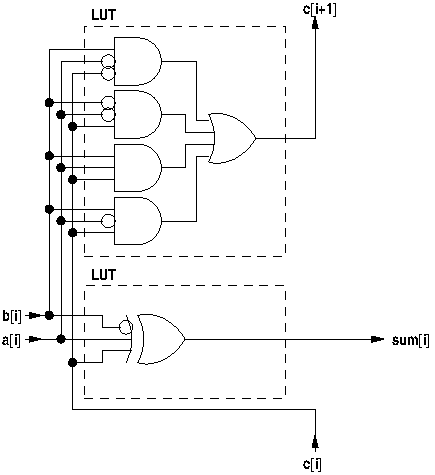
\includegraphics{sub_ncc}

    As in the case of {\bf add(}) the variables {\bf add\_sub\_use\_lut}
    and {\bf cpld\_use\_lut}, which are public static variables in
    ThreePL.jj, select whether the combinatorial logic is expressed
    as a LUT or a combination of AND, OR, XOR and INV elements.

\subsection{decrementer}

    The decrementer method is only used for an up/down counter ({\bf
    method cb()}). It is derived from the code for method {\bf sub()}
    with the second input {\bf b} omitted and the carry input connected
    to the inverted {\bf enable} input. Thus when {\bf enable} is low the output
    is the same as the input {\bf a} and when {\bf enable} is high the
    output is {\bf a} - 1. The result is the same width as the input,
    not one greater.

    {\bf Warning} - method {\bf cb()} only calls {\bf decr()} if its
    sixth parameter {\bf down} is not null and its second parameter {\bf
    dwn} is true. This does not occur in the code as it currently is and
    hence {\bf decr()} has never been called and its validity has not
    been tested!


\subsection{adder/subtracter}

    This adder/subtracter is used internally in XFunctions.java for the
    implementation of division. It is also used for the inbuilt
    function {\bf addsub()} (called in XTDECode.java.TDEOPERATOR()).
    It provides the ability to gate the second operand so that the
    add/subtract is supressed and it XORs the carry input with an
    input Net so that the carry input can be inverted. For addition
    this will increment the sum with no extra logic.

    \begin{lstlisting}[gobble=4, language=java]
        public Net[] addsub (Net[] a, Net[] b, Net add, Net igb, Net xci, boolean asigned, boolean bsigned) {
            if (needCPLDarith())
                    throw new ExEx("CPLD CODE ERROR - addsub() used");

            int     awid = a.length + ((!asigned && bsigned) ? 1 : 0);
            int     bwid = b.length + ((asigned && !bsigned) ? 1 : 0);
            int     size = Math.max(awid, bwid) + 1;
            Net[]   di = new Net[size];
            Net[]   psd = new Net[size]; // partial sum/difference
            Net[]   sd = new Net[size];  // sum/difference
            Net[]   c = new Net[size];   // carries

            a = sig_expand(a, size, asigned);
            b = sig_expand(b, size, bsigned);
            if (xci.isConnected(Net.LO))
                c[0] = AND(INV(add), igb);
            else
                c[0] = AND(XOR(INV(add), xci), igb);
            for (int i=0 ; i<size ; i++) {
                if (igb.isConnected(Net.LO))
                    psd[i] = a[i];
                else if (igb.isConnected(Net.HI)) {
                    if (add.isConnected(Net.LO))
                        psd[i] = XOR(a[i], INV(b[i]));
                    else if (add.isConnected(Net.HI))
                        psd[i] = XOR(a[i], b[i]);
                    else
                        psd[i] = OR(AND(add, XOR(a[i], b[i])), AND(INV(add), XOR(a[i], INV(b[i]))));
                } else {
                    if (add_sub_use_lut)
                        psd[i] = LUT("(!I0*I1)+(I0*(I3*(I1^I2)+!I3*(I1^!I2)))", igb, a[i], b[i], add);
                    else
                        psd[i] = OR(    AND(INV(igb), a[i]),
                                        AND(igb, OR(    AND(add, XOR(a[i], b[i])),
                                                        AND(INV(add), XOR(a[i], INV(b[i]))))));
                }
                if (igb.isConnected(Net.LO))
                    di[i] = Net.LO;
                else if (igb.isConnected(Net.HI))
                    di[i] = a[i];
                else
                    di[i] = MULT_AND(a[i], igb);
                if (i != (size-1))
                    c[i+1] = MUXCY(psd[i], di[i], c[i]);
                sd[i] = XORCY(psd[i], c[i]);
            }
            return(sd);
        }
    \end{lstlisting}

    The implementation does not provide a non-carry-chain version
    for CPLDs, hence the check on entering the method.

    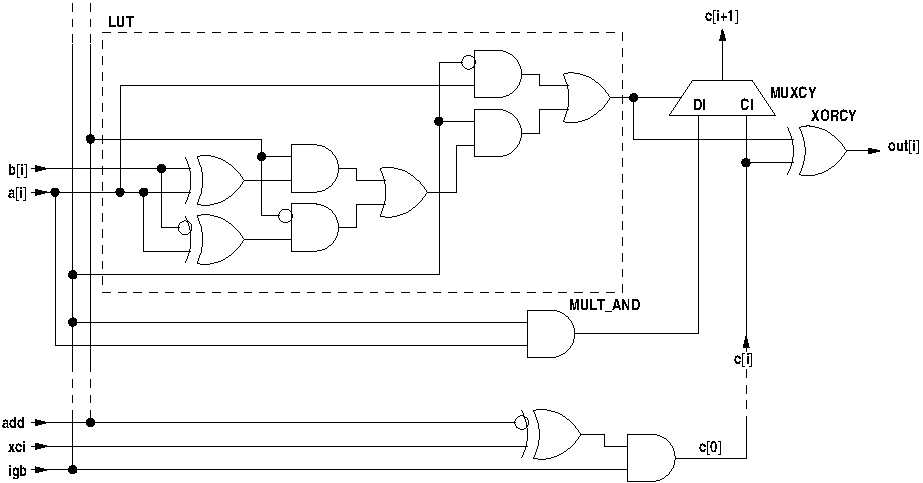
\includegraphics{addsub}

    Note that if {\bf igb} is low {\bf a[i]} is passed through the LUT
    and the XORCY unchanged. The LUT function passes a[i] through to
    its output and the XORCY has a low from the carry on its other input.
    The carry chain is low along its length as {\bf c[0]} is forced low
    and the {\bf DI} inputs to the MUXCYs are forced low.

    The {\bf add} input inverts the {\bf b[i]} inputs and also controls
    the carry input, {\bf c[0]} (low for add, high for subtract). {\bf
    xci} inverts that {\bf c[0]} input.

    The expression represented in lines 37 and 39 and in the logic
    diagram could be written more concisely but it does not matter as it
    would be converted to the same function of four variables in the LUT
    in either case.

\subsection{ALU}

    The {\bf alu()} code is very similar to the {\bf addsub()} with
    the following exceptions -
    \blist
    \item   the {\bf xci} input and function is omitted
    \item   it has an {\bf iga} input instead of {\bf igb}, i.e. it
            gates the {\bf a} input to give output = b when asserted
    \item   there is a {\bf dsp} parameter which if true and the device
            is a Virtex5 or later will implement the ALU in a DSP
            block instead of using CLB logic.
    \blend
    The output Net array is one larger than the largest operand.


\subsection{incrementer/decrementer}

    This method is only called in one place, method cb() in class
    XFunctions. It increments or decrements its operand according to the
    second argument. It is derived from method {\bf addsub()}. The
    output Net array is the same size as the operand (first argument).


\subsection{signed and unsigned multipliers}

    The multiplier method, {\bf mul()}, is divided into four sections
    depending on FPGA type -
    \blist
    \item   XC3S, XC2V or XC2VP
    \item   XC4V
    \item   XC5V or XC6V
    \item   others
    \blend

    This method must be called such that if the operands are of
    different sizes the first must be the larger except in the case
    where one operand is a constant in which case the constant operand
    is the second one.

    For Spartan 3, Virtex 2 or Virtex 2 Pro the MULT18X18 is used. Up to
    four multipliers can be combined to give a maximum of 35 by 35 bits
    signed (See Xilinx application note XAPP467 and Xilinx white paper
    WP277). Since the MULT18X18 performs signed multiplication, unsigned
    operands cannot use the top bit, which must be 0 to give a positive
    sign. For this reason operand size checks are different for signed
    and unsigned operands.

    For the Virtex 4 a MULT18X18 is created but this will later be
    converted to a DSP48 by the place-and-route software.

    For Virtex 5 and Virtex 6 a single MULT25X18 is used. This size
    was deemed sufficient and larger multipliers using combined
    MULT25X18 elements have not been coded.

    For other types of FPGA (Spartan 2, Virtex, Virtex E) a multiplier
    is constructed using cascaded adders. This usually results in
    considerable signal path lengths through combinatorial logic and
    hence this form of multiplier will usually only work at relatively
    low clock frequencies. All current FPGA platforms have hardware
    multipliers and this combinatorial logic is only included for
    obsolete FPGAs still in use. There is a library, {\bf multlib.3pl},
    which implements pipelined multiplies which will operate at
    high clock frequencies (which of course have multi-cycle latency).

    If the operands are mixed signed and unsigned, the unsigned operands
    has a (zero) sign bit added. If either operand is signed method {\bf
    muls()} is called, otherwise {\bf mulu()} is called. These methods
    both call method {\bf mul\_add()} for each bit of the second
    operand. If the second operand is a constant then adders are only
    created for the 1 bits and the partial product is passed on
    unchanged for 0 bits. For a constant multiplier with only a few 1
    bits the resulting multiplier will have a significantly smaller
    delay than for the case of a variable multiplier.


\subsection{signed and unsigned divider/remainder}

    Division method {\bf div()} and remainder method {\bf rem()} call the combined
    quotient/remainder method {\bf quotrem()}. {\bf quotrem()} in turn calls {\bf
    quotrems()} for signed operands or {\bf quotremu()} for usigned operands. {\bf
    quotrems()} calls recursive method {\bf part\_sdiv()} and {\bf quotremu()}
    calls recursive method {\bf part\_udiv()}. These recursive methods construct
    staged adders and subtracters to carry out the division. These stages are not
    pipelined and hence the use of division or remainder operations is likely to
    result in high path delays. These are probably not practical and have been
    included for completeness.

    
\subsection{numerical comparators}

    Methods {\bf eqones()} and {\bf eqzeros()} test for all ones and all zeros
    respectively and are implemented using AND/OR gates. For wide inputs these
    will be optimised using MUXes or carry chains.     Methods {\bf eq()} and {\bf
    ne()} compare operands and are similarly implemented to the methods above.

    Magnitude comparisons gt, ge, lt and le are all implemented using only the
    method {\bf ge()} with suitable operand order and output inversion. This is
    implemented as subtraction using the carry chain if necessary, the final carry
    bit giving the result.



\subsection{combinatorial RAM and ROM}

    Methods {\bf sram1()}, {\bf sram2()} and {\bf srom1()} build combinatorial
    RAMS (CLB RAM) of various widths and depths calling methods {\bf RAM\_1()},
    {\bf RAM\_2()} or {\bf ROM\_1()} in class XElements().


\subsection{registered output RAM}

    Methods {\bf rram1()} and {\bf rram2()} call method {\bf ramallocate()}
    in the FPGA class. This method creates a list of class RamBlock to map
    the memory across the required number of blocks and then traverses that list
    calling RamBlock.RAMB() in class RamBlock to generate the blocks elements.
